\documentclass[xcolor=dvipsnames,beamer,compress]{beamer} %handout,notes=show
% \documentclass[xcolor=dvipsnames,beamer,compress]{beamer} %handout,notes=show

\usepackage{textcomp}
\usepackage[utf8x]{inputenc}
% \usepackage{default}
\usepackage[czech]{babel}
\usepackage{graphicx}
%  \usepackage[pdftex]{hyperref}
\usepackage{url}
\usepackage{pgfpages}
% \usepackage{verbatim}
\usepackage[absolute,overlay]{textpos}

%%%%%%%%%%%%%% Listings %%%%%%%%%%%%%%%%%
\usepackage[final]{listings}

\definecolor{lightGrey}{RGB}{250,250,250}
\definecolor{darkGrey}{RGB}{100,100,100}
\lstdefinelanguage{psmap}
{morekeywords={scale, mapinfo, maploc, where, end, font, fontsize, color,
border, raster, width, paper,
vpoints, vareas, vlines, symbol, size, rgbcolumn, sizecolumn, cwidth,
rotatecolumn, },
morekeywords=[2]{y, n, none},
morecomment=[l]{\#},
}
\lstdefinestyle{psmap}{
    language=psmap,
    basicstyle={\sffamily\small},
    keywordstyle=[1]{\bfseries},
    keywordstyle=[2]{\color{black}},
    commentstyle={\itshape},
    }
        
        
\lstdefinestyle{script}{
    language=bash,
    basicstyle={\ttfamily\footnotesize},
    keywordstyle={\bfseries},
    commentstyle={\itshape},
    frame=lines,
    backgroundcolor=\color{lightGrey}
    }
    \lstnewenvironment{psmap}[1][]
    {\lstset{style=psmap,
    #1}}
    {}



\usepackage{color}

% \usetheme{Warsaw}
% \usetheme{Madrid}
\usetheme{Szeged}

% \useoutertheme[subsection=false]{miniframes}
\definecolor{zelena}{RGB}{143,172,83}

\usecolortheme[named=zelena]{structure}
% \usecolortheme[named=PineGreen]{structure}
% \setbeamertemplate{navigation symbols}{}
\useinnertheme{rectangles}
% \setbeamertemplate{blocks}[default]

\setbeamercolor{separation line}{bg=zelena}
\setbeamercolor{frametitle}{fg=OliveGreen}
\setbeamercolor{title}{fg=OliveGreen}
\setbeamercolor{block title}{fg=OliveGreen}





\title[GUI for composing hardcopy map outputs in GRASS GIS]
{Graphical User Interface for composing hardcopy map outputs in GRASS GIS}
%\subtitle{\pdforstring{}{}}

\author[A. Kratochv\'{\i}lov\'{a}]
{Anna Kratochv\'{\i}lov\'{a}  }

\institute[FCE CTU in Prague]{Czech Technical University in Prague \\ Faculty of Civil Engineering \\
\vspace{12pt}

\includegraphics[width=3cm]{Grass_GIS}}


% \AtBeginSection[]{\begin{frame}\frametitle{Obsah}%
% \tableofcontents[currentsection ]\end{frame}}
% \AtBeginSubsection[]
% {
%   \begin{frame}<beamer>
%   \frametitle{Obsah}
%   \tableofcontents[currentsection,currentsubsection]
%   \end{frame}
% }

\setbeamercovered{transparent}

% \setbeamercolor{block title}{bg=orange}
\setbeamercolor{block body}{bg=SpringGreen!30}

\newcommand{\normalniradky}{%
% \setlength{\parskip}{\oldparskip}
\renewcommand{\baselinestretch}{1.0}%
\selectfont % baselinestretch takes effect after new font is selected
}

\newcommand{\roztazeneradky}{%
% \setlength{\parskip}{0.8ex plus 0.4ex minus 0.1ex}%
\renewcommand{\baselinestretch}{1.3}%
\selectfont
}
%%%%%%%%%
\newif\ifnotes
% \notestrue


\ifnotes
\setbeamertemplate{note page}[compress]
\setbeamerfont{note page}{size=\large}
 \setbeameroption{show only notes}
\usepackage{pgfpages}
\pgfpagesuselayout{2 on 1}[a4paper,border shrink=5mm]
\else
\setbeameroption{hide notes}
\fi
%%%%%%%%%%%%%%%%%%%%%%%%%%%%%%%%%%%%%%%%%%%%%%%%%%%%%%%%%%%%%%%%%%%
\begin{document}


\frame{\titlepage
\note{}
}
\logo{
\includegraphics[width=0.05\textwidth]{Grass_GIS}}

 \begin{frame}{Contents}
 \tableofcontents
 \end{frame}
\section{Introduction}
\begin{frame}{Basic information about this project:}
%  Basic information about this project:
\roztazeneradky
 \begin{itemize}
  \item realized within bachelor thesis
  \item mentor Ing. Martin Landa
  \item development started in January
  \item now available in GRASS AddOns
 \end{itemize}

 \end{frame}

\begin{frame}{Project motivation}
% \begin{itemize}
GRASS GIS---tool intended for data analysis, not for cartography\\
\bigskip
\begin{center}
$\Longrightarrow$ unsatisfactory situation in creating map outputs                                                                  \end{center}
% \end{itemize}
\begin{block}{Module \emph{ps.map}}
\begin{itemize}
  \item specialized tool for creating hardcopy maps
  \item input---text file with mapping instructions
  \item output---PostScript format
\end{itemize}

\end{block}

\end{frame}

\section{Module ps.map}


\begin{frame}{Using ps.map}
\roztazeneradky
\begin{block}{ps.map---not easy to use:}
\begin{itemize}
\item knowledge of the names of instructions and their usage
\item inconvenient determining of object's position on paper\\
(pencil, paper and calculator are often needed)
\item takes time to get the intended result
\end{itemize}
\end{block}
\end{frame}


\begin{frame}[fragile]{Mapping instructions}
\begin{itemize}
  \item about 30 instructions
  \item most instructions have a few subcommands
\end{itemize}

\begin{block}{Simple example}
\begin{psmap}
  paper a4
      end
  raster aspect
  vlines streams
      width 1
      color 0:0:255
      end
  end
\end{psmap}
\end{block}
\end{frame}


\begin{frame}{ps.map functionality}
% \roztazeneradky
Basic elements used in cartographic output
\begin{itemize}
  \item raster, vector layers
  \item map legend (raster and vectors separately)
  \item scale bar
  \item text
  \item grid
  \item points, lines, rectangles
  \item EPS images
\end{itemize}

\end{frame}

\begin{frame}{ps.map inconveniences}
 \roztazeneradky
\begin{itemize}
\item only one raster layer
\item numeric scale only within mapinfo
\item some accented characters not supported (encoding Latin1)
\item inconsistencies in used coordinates systems, reference points
\item named colors \texttimes\ RGB (partly solved)

\end{itemize}

\end{frame}

\section{GUI for ps.map}
\begin{frame}{GUI for ps.map}
% \roztazeneradky
\begin{itemize}
\item Map composing with ps.map is not comfortable enough
\item GUI is needed
% \item  \emph{Hardcopy Map Output Utility} (also called \emph{wx.psmap}) developed
\end{itemize}
\hspace*{1cm} $\Rightarrow$\ \emph{Hardcopy Map Output Utility} (also called \emph{wx.psmap})

\begin{block}{Main advantages}
\begin{itemize}
\item interactive positioning of map elements
\item no need to know ps.map instructions
\item preview of result
% \item follows the appearance of GRASS wxGUI
\end{itemize}
\end{block}

\hspace*{1cm} $\Rightarrow$ makes the map composing easier and faster
\end{frame}

\begin{frame}{Implementation basics}
\begin{block}{Basic schema}
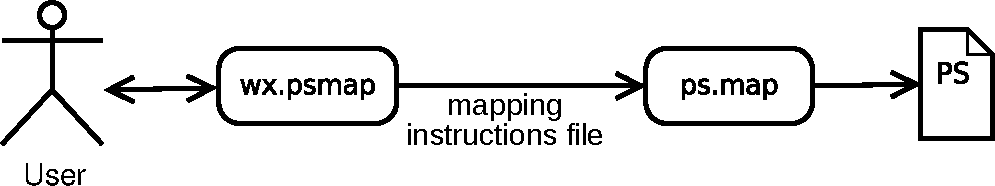
\includegraphics[width=0.9\textwidth]{./diagram.pdf}
\end{block}
\bigskip
\begin{block}{Programming language, library}
\begin{itemize}
\item programming language \emph{Python}
\item GUI toolkit  \emph{wxPython}
\end{itemize}
\end{block}
\end{frame}

\begin{frame}{\emph{wx.psmap} possibilities}
\roztazeneradky
\begin{itemize}
\item wx.psmap  supports major part of ps.map instructions\\
(and the most important)
\begin{itemize}
\item raster and vector layers
\item map legend (raster and vector)
\item scale bar, text
\item map info (scale, extent)
\end{itemize}
\end{itemize}
\end{frame}


\begin{frame}{\emph{wx.psmap} possibilities}
\roztazeneradky
\begin{itemize}
\item wx.psmap makes map composing more comfortable
\begin{itemize}
\item zoom, pan
\item preview of result
\item ability to read configuration file
\item region is set internally
\item output formats:
    \begin{itemize}
      \item PS
      \item PDF (if ps2pdf is available)
      \item configuration file with basic info in header
    \end{itemize}
% PS, PDF (if ps2pdf is available), configuration file

\end{itemize}
\end{itemize}
\end{frame}

\begin{frame}{Region in wx.psmap}
\begin{itemize}
\item ps.map draws data from current region (set via \emph{g.region})
  \item wx.psmap sets region internally (doesn't affect current region)
  \item several options:
      \begin{itemize}
        \item match raster/vector map extent
        \item use named region
        \item use current region
        \item region computed from map center and scale
      \end{itemize}
  \item region settings are written in configuration file as a comment
\item this comment is used when reading configuration file
\end{itemize}

\end{frame}


\begin{frame}{Draft \& Preview mode}
\begin{block}{Draft mode}
\begin{itemize}
  \item for composing map output interactively
  \item map elements are represented by colored rectangles
\end{itemize}
\end{block}

\begin{block}{Preview mode}
\begin{itemize}
\item preview of result (lowered quality)
\item non-interactive mode
\end{itemize}
\end{block}
\end{frame}

\begin{frame}{Draft \& Preview mode}
\begin{columns}[c]
\column{0.5\textwidth}
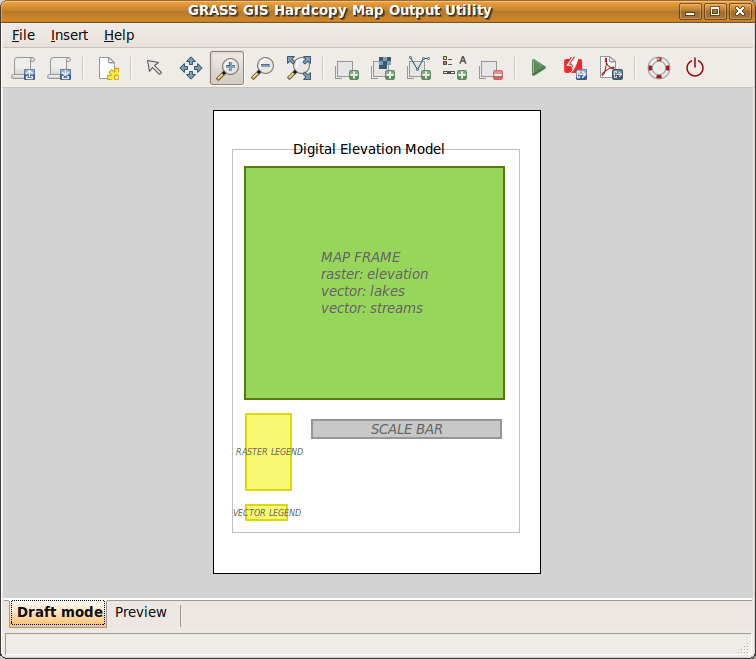
\includegraphics[width=\textwidth]{./screenshoty/draft.png}

\column{0.5\textwidth}
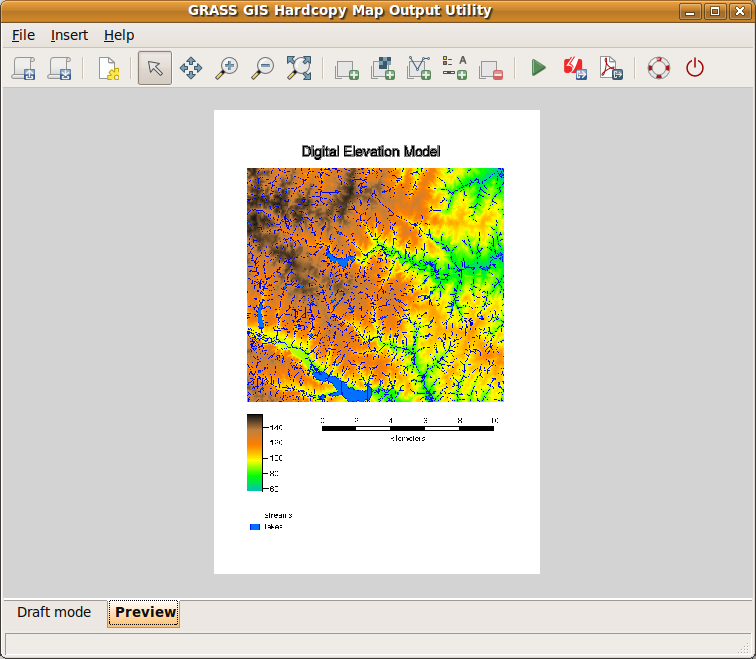
\includegraphics[width=\textwidth]{./screenshoty/vysledek.png}
\end{columns}

\end{frame}

\begin{frame}{Limitations}
\begin{itemize}
\item 
wx.psmap is limited by ps.map's functionality
and interface
\end{itemize}
\begin{block}{Consequences}
\begin{itemize}
  \item inaccurate size of map elements in draft mode (depends on font size and other parameters)
  \item resizing of map elements is not supported (except for map frame)
\end{itemize}
\end{block}
\end{frame}


\section{Video demonstration}
\begin{frame}{Video demonstration of wx.psmap}
\begin{block}{}
\begin{itemize}
\item\href{basic.avi}{Basics}
\item\href{decorations.avi}{Adding map elements}
\item\href{elevation.pdf}{Result}

\end{itemize}
\end{block}
\hyperlink{conclusion}{\beamergotobutton{Conclusion}}
\end{frame}

% just for sure
\begin{frame}{Draft mode}
\begin{center}
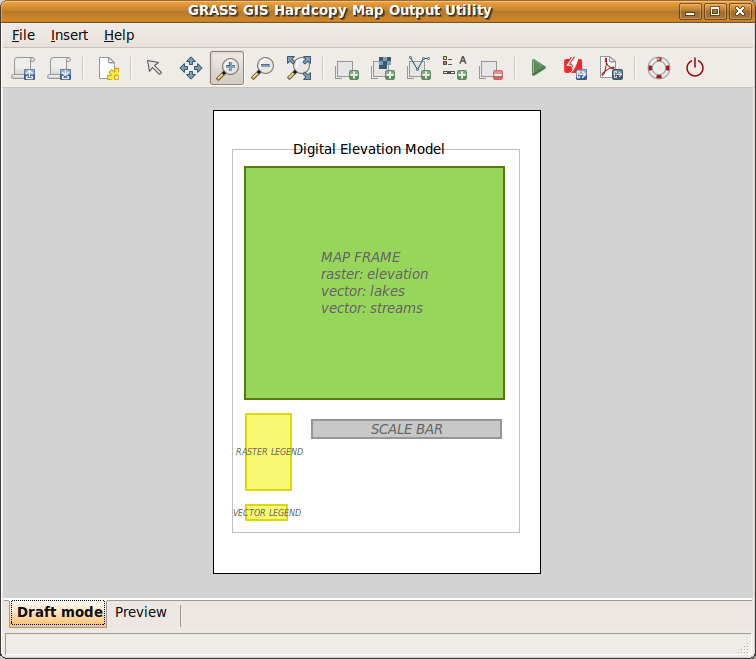
\includegraphics[height=0.8\textheight]{./screenshoty/draft.png}
\end{center}
\end{frame}

\begin{frame}{Dialog window---vector layers}
\begin{center}
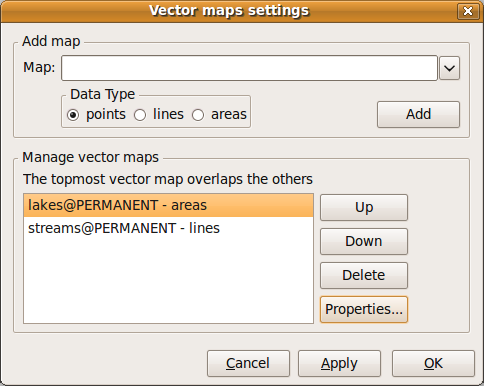
\includegraphics[height=0.8\textheight]{./screenshoty/vector.png}
\end{center}
\end{frame}

\begin{frame}{Dialog window---scale bar}
\begin{center}
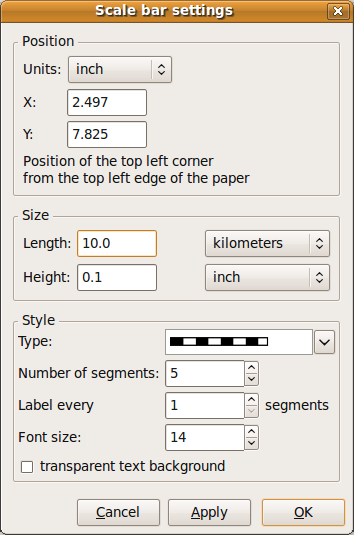
\includegraphics[height=0.8\textheight]{./screenshoty/scalebar.png}
\end{center}
\end{frame}

\begin{frame}{Dialog window---text}
\begin{center}
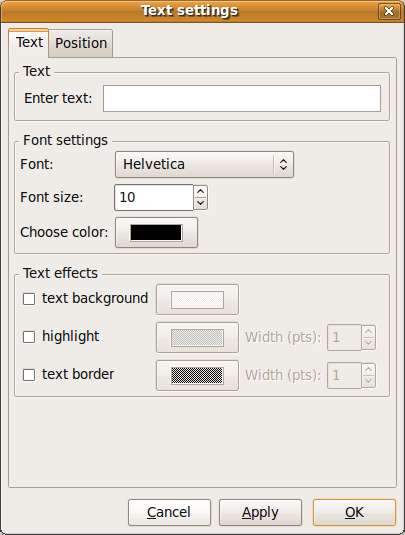
\includegraphics[height=0.8\textheight]{./screenshoty/text.png}
\end{center}
\end{frame}

\begin{frame}{Preview}
\begin{center}
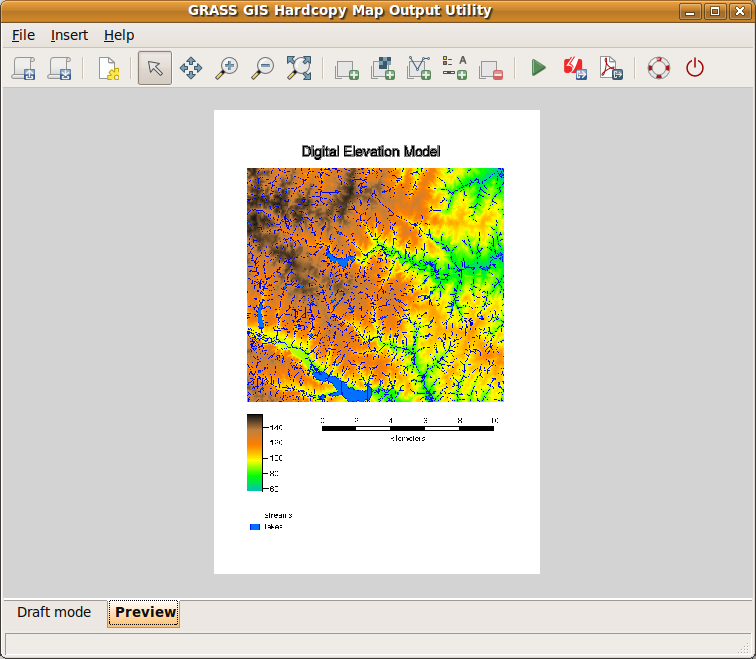
\includegraphics[height=0.8\textheight]{./screenshoty/vysledek.png}
\end{center}
% \note{ }
\end{frame}

\section{Conclusion}
\begin{frame}[label=conclusion]{Conclusion}
\begin{block}

\begin{itemize}
\item wx.psmap is available in GRASS AddOns
\item wx.psmap is planned to be the part of  GRASS GIS 6.4.2
\item it is intended to continue with the development (support instructions like grid or eps)

\end{itemize}
\end{block}
\end{frame}

\end{document}
